%%%%%%%%%%%%%%%%%%%%%%%%%%%%%%
% 	   美赛模板,正文部分		 
%          PAPER.tex         
%%%%%%%%%%%%%%%%%%%%%%%%%%%%%%

\documentclass[12pt]{article}

% 请在此填写控制号、题号和标题,年份不需要填(自动以当前电脑时间年份为准)
\usepackage[1925254]{easymcm}\problem{D}   
\usepackage{palatino} % 这个是COMAP官方杂志采用的字体,如不需要可注释掉,以使用默认字体
\title{Mission Evacuation:Possible}  % 标题

% 如您参加的是ICM(即选择了D/E/F题),请使用以下的命令修改Summary Sheet题头
\renewcommand{\contest}{Interdisciplinary Contest in Modeling (ICM) Summary Sheet}

% 正文开始


\usepackage[T1]{fontenc}
\usepackage[skip=1ex]{caption}
\usepackage{booktabs,tabularx}
\usepackage{siunitx}
\newcolumntype{C}{>{\centering\arraybackslash}X}
\newcommand{\mcx}[2]{\multicolumn{#1}{>{\hsize=\dimexpr#1\hsize
                                        + #1\tabcolsep + #1\tabcolsep\relax}C}{#2}}
\newcommand{\mcone}[1]{\multicolumn{1}{C}{#1}}





\begin{document}
%%%%%%%%%%%%%%%%%%%%%%%%%%%%%%%%%%%%%%%%%
%%            请在此填写摘要            %%
%% 请勿编译/排版此文件,请编译PAPER.tex!  %%
%%%%%%%%%%%%%%%%%%%%%%%%%%%%%%%%%%%%%%%%%
\begin{abstract}\small
To evacuate visitors, we proposed an adapted Graph Theory
Model with strong adaptability, which endows vertices with weight to show congestion degree. Simultaneously, we utilized the Cellular Automata(CA) theory to simulate the behavior of visitors,and add them to our graph as moveable and dynamic point cluster.

For potential bottlenecks' identity, we separately abstracted 
spacious space and narrow space  to edge and vertex
(Potential Bottleneck's Candidate,PBC) 
based on crowd flow density-velocity model and abundant observation data.We innovatively redefined the weight value of Graph Theory as PBC's throughput to show the congestion degree. Subsequently we found that the  the building's tridimensional character can be indirectly reflected by the existing parameters. Thus, our team creatively and reasonably abstracted the complex three-dimensional model into a big two-dimensional planar graph, simplifing the problem.  

For visitors' diversity, we simulated a wide variety of visitors by specifying diverse cellular rules. The differences among visitors are mainly reflected on moving velocity and evacuation route's choice.Also, we noticed that the Louvre, as an international tourist attraction, has lots of visitors from different countries,
We investigated the proportion of different languages and then put forward some suggestions.

For potential threats' influence,our model combines the advantages 
of Cellular Automata and Graph Theory 
by making cellular rules based on adjacency matrix, which brings strong adaptability. Through the modification of Cellular Automata's rule and the CRUD(create, read, update, delete) operations on the graph edge and vertex, we can efficiently complete the simulation and optimization of various potential threats.   

For additional exits' utilization, we believed that nearby crowd flow density, 
overall crowd flow density, emergency degree and security are the primary 
determinants of whether to open addtional exits(AE) or not and provided a 
threshold calculation method. 
Meanwhile, with regards to emergency personnel, 
we will exclusively open the AE considering  congestion degree and optimal convenience. 
In our model, we initially represent the unpublicized exits by the unreachable vertices, and when a AE is opened, its adjacency matrix value will be reassigned accordingly. 
 
For high technology's application, we designed two different apps separately for staffs and visitors,emphasizing real-time information acquisition. It is hoped that the monitoring of potential bottlenecks, the automatic estimate of the congestion degree as well as the optimization of evacuation routes can be implemented by machine learning algorithm.

For the experiment part, we utilized Java to design model's visualization program, 
which clearly tell the congestion degree of every vertex. Then we adjusted the visitor number, AE number and staff number in our model and got the result evacuation time ranging among 614 to 2435 seconds. Then we carried out sensitivity analyses with these three factors .

At last we offered recommendations to the museum's leaders and discussed our model's strengths and weaknesses as well as adaption in other large buildings.  

 
   
     \vspace{5pt}
     \textbf{Keywords}: Graph Theory,weighted vertex,Cellular Automata,two-dimensional abstract,\\strong adaptability,GUI

\end{abstract}




%%%%%%%%%%%%%%%%%%%%%%%%%%%%%%%%%%%%%%%%%%
% 如不理解以下部分中各命令的含义,请勿修改! %
%%%%%%%%%%%%%%%%%%%%%%%%%%%%%%%%%%%%%%%%%%

%---------以下生成sheet页----------
% 下面的语句可调整全文行距为标准值的0.6倍,请自行使用
% \renewcommand{\baselinestretch}{0.6}\normalsize
\maketitle  			% 生成sheet页
\thispagestyle{empty}   % 不要页眉页脚和页码
\setcounter{page}{-100} % 此命令仅是为了避免页码重复报错,不要在意

%---------以下生成目录----------
\newpage
\tableofcontents
\thispagestyle{empty}   % 不要页眉页脚和页码
\newpage

%---------以下生成正文----------
\setlength\parskip{0.8\baselineskip}  % 调整段间距
\setcounter{page}{1}    % 从正文开始计页码
\pagestyle{fancy}		% 摘要请到ABSTRACT.tex中填写

\section{Introduction}
\subsection{Problem Background}
France has seen repeated street and violent protests over the last two months–a scenario that could become more mainstream worldwide, the Edelman Trust Barometer Report warned Sunday.\cite{1} In the capital, the protests left charred car frames, shattered shop windows and vandalized monuments — as well as a presidency in crisis. This makes us to reconsider the existing evacuation plans at many popular destinations such as the Louvre.  

According to the official data from the Louvre website, we found that the Louvre recorded a sharp increase in visitor attendance from January to December 2018, with 10.2 million visitors (+25\% compared to 2017)\cite{2} The themed Entertainment Association report cited by Le Parisien claimed that after being once overtaken by the National Museum of China and the National Air and Space Museum, the Louvre Museum has re-emerged as the most visited museum.\cite{3}

Located in central Paris with thousands of visitors daily, it is rather crucial and nonnegligible for the emergency management agency of the Louvre to figure out optimal evacuation plan to have all the occupants leave the buildings as quickly and safely as possible in emergency. 



\subsection{Problem Restatement}

In the last couple of years, the number of the malicious terror attacks in France has increased a lot. Under this circumstance, the reevaluation of the emergency evacuation plans at places with high visitor flow volume is rather crucial for safety. Our model was built primarily for helping with the design process of evacuation plans at the Louvre in Paris, France.  

To have all the visitors evacuate the Louvre as quick and safe as possible, our model should be able to fulfill 5 tasks as follows:


\begin{enumerate}
\item Visitor are diverse.The number of the visitor in the museum doesn't remain the same. On the contrary, it varies throughout the day and year due to a serious of factors.The diversity of the visitors, say speaking multiple languages, group visit, infants, the elderly people and visitors with disability.
\item Additional Exits' Utilization.Considering how to probably utilize the additional exits, taking into account the potentialsecurity danger or other threats caused by the lack of security safeguard in theunannounced exits.And How to allow emergency personnel to enter the building at the firsttime to provide assistance in the emergency.
\item Identity the Potential Bottlenecks.Which factors can determine a potential bottlenecks and how do we find them and optimize them?Validate the calculated models and discuss how to implement the models in possible and achievable ways to evacuate the visitors.
\item Various types of potential threats.The modeling process by our team should be able to address a broad set of considerations and various types of potential threats. Regenerate a new and optimal solution when the type of threats change and furnish a range of feasible and optimal options .
\item Combine with high technology.Considering how to utilize the existing intelligent science and technology technology, including apps such as Affluences, cloud computing , machine learning etc, to facilitate our evacuation models.
\end{enumerate}

Apart from the above tasks, we also need to propose policy and recommendation for the emergency management of the Louvre which should include indispensable and applicable crowd management procedures for the safety of visitors' sake. Meanwhile, we should consider our evacuation model's applicability at other crowd and large buildings.






\subsection{Overview of our work}
According to the requirement of the problem, we proposed a graph theory 
model with strong adaptability by the means of transforming the weighted 
undigraph. On the basis of the construction principle of particle in 
physics, we gave the weight to the vertex for the purpose of presenting 
the potential bottlenecks' crowding degree. Simultaneously, we utilized 
the Cellular Automata(CA) theory to simulate the behavior of visitors 
which existed as a moveable and dynamic point cluster in the graph.

For task 1, we simulated multiple kinds of the visitors by specifying different parameters of the Cellular Automata(CA). Meanwhile, we studied the effect of the changing number of the visitors on model results. Considering the diversity of languages spoken by the visitors, several effective solutions were proposed by our team's research and calculation results at the end.

For task 2, we restricted the use of the AE by visitors and discussed the issue about how and when to utilize the AE. 

For task 3, we first discussed the three-dimensional characteristic of the Louvre Museum. Then we discovered a better approach to the modeling process which utilized the two-dimensional planar graph based on the abstraction of specific objects such as staircases and elevators. Soon afterwards, we abstracted the capacious and unimpeded hall to edge and the narrow and crowded space was also abstracted to vertex, namely PBC (Potential Bottlenecks Candidates) on the basis of the density-velocity parametric representation model to expose potential bottlenecks. 

For task 4, we discussed the parameters and the potential influencing 
factors on the model variously. By means of the modification cellular rule and the four 
operations separately named as create, read, update and delete(CRUD) based 
on the Graph theory, it is rather simple and efficient to accomplish the simulation and optimization of various potential emergencies.

For task 5, we designed two different apps for the emergency personnel or the museum officials and the visitors. It is hoped that during the development of our apps, the real-time monitoring of the PB, the automatic estimate of the congestion degree as well as the optimization of evacuation routes can be implemented by means of the machine Learning algorithms and AI processing ability of our apps.

On the basis of the aforementioned work and analyses, our team proposed abundant feasible and operable policies and recommendations for the emergency management of the Louvre. Additionally, we discussed and analyzed the practicability of our models' application in other large and crowded buildings such as the Louvre in the last section of our paper.




\section{Preparation of the Models}
\subsection{Assumptions}
\begin{itemize}
	\item \textbf{Assumption \uppercase\expandafter{\romannumeral1}:}Under emergent situations, all the visitors in the Louvre Museum will orderly follow the instructions from staffs.\\
 
	\item \textbf{Assumption \uppercase\expandafter{\romannumeral2}:}All the data and information we found about the Louvre Museum is valid, authentic and effective.
	
	\item \textbf{Assumption \uppercase\expandafter{\romannumeral3}:}All the correlative electronic products and communication technology will not be damaged and can still be utilized to evacuate the visitors as quickly and safely as possible.
	\item \textbf{Assumption \uppercase\expandafter{\romannumeral4}:}The emergency personnel used for the assistance and aid of the evacuation process are adequate and are able to enter work-mode quickly and rapidly.  
	\item \textbf{Assumption \uppercase\expandafter{\romannumeral5}:}The speed of visitors moving in the wide exhibition hall will not be affected by the exhibits.
	\item \textbf{Assumption \uppercase\expandafter{\romannumeral6}:}All the staff helping evacuation are trained which means they know all the available exits and have some real-time means of communication.
\end{itemize}






\subsection{Notations}
The primary notations used in this paper are listed in \textbf{Table \ref{tb:notation}}.




\begin{table}[htbp] 
\begin{center}
\caption{Notations}
\begin{tabular}{cl}
	\toprule
	\multicolumn{1}{m{3cm}}{\centering Symbol}
	&\multicolumn{1}{m{8cm}}{Definition}\\
	\midrule
	D$_{ij}$ &the distance between the door i and the door j \\
        i &the door's relative number is i \\
        j &the door's relative number is j \\
        v$_{1}$ &the moving speed of visitors without congestion \\
		v$_{2}$ &the moving speed of visitors in the case of congestion \\  
		t &the total time of evacuation \\
		t$_{0}$ &the time people aware of emergency \\ 
        t$_{1}$ &the time it takes to move from one door to another \\
        t$_{2}$ &the queuing time \\
        T$_{ij}$ &the time it takes to move from PBC i to PBC j \\
        T &the throughput of the PBC \\
        w &the effective width of the PBC \\
        $\rho$ &the crowd flow density \\
        $\rho$$_{1}$ &the horizontal linear density \\
		$\rho$$_{2}$ &the vertical linear density \\
		PB           &the potential bottlenecks\\
		PBC          &the potential bottlenecks' candidates\\
		AE           &the additional exits\\
	\bottomrule
\end{tabular}\label{tb:notation}
\end{center}
\end{table}

\section{The Model Process}
\subsection{Our Model}
In the process of working out the visitor's evacuation issue when emergency circumstances happen in the Louvre, we discovered that the intricate and complex architectural style and construction of the Louvre itself made it rather difficult when simulating its evacuation model. We have to admit that, in any case, the scene reconstruction of a magnificent and crowd 198-hectare large-scale building is rather time consuming, resource demanding as well as insignificant. Hence, based on the reasonable abstraction and moderate simplification of the modeling process, we presented the framework of the Louvre evacuation model by keeping the key influencing factors.

\subsubsection{Influencing Factors}
First of all, we carried out a detailed and comprehensively analysis of the potential influencing factors when the building is under evacuation in case of emergency. The primary influencing factors are as follows:


\begin{table}[ht]
	\begin{center}
	\begin{tabular}{p{4cm}<{\centering}|c|c|p{3cm}<{\centering}} \hline
		\multirow{7}{*}{ Personnel Factor }
		 & No. & Affecting factors &  Affecting result \\ \hline
		 & 1 & Staff's guidance  &   t$_{0}$ t$_{2}$   \\ \cline{2-4} 
		 & 2 & Crowd flow density  &   $\rho$   \\ \cline{2-4} 
		 & 3 & Visitor's walking speed  &  t$_{1}$   T$_{ij}$  \\ \cline{2-4} 
		 & 4 &Visitor's language  &     t$_{0}$  \\ \cline{2-4}
		& 5 & Visitor's type  &   t$_{1}$ t$_{2}$   \\ \cline{2-4} 
		& 6 & Visitor's risk consciousness  &  t$_{0}$ t$_{2}$   \\ \hline
		\multirow{6}{*}{Architectural Factor}
		  & 7 & Evacuation distance  &   T$_{ij}$    \\ \cline{2-4} 
		& 8 & The number of the exits  &    t  \\ \cline{2-4} 
		  & 9 & The structure and layout  &  w T    \\ \cline{2-4}
		  & 10 & The number of the storeys  &   t   \\ \cline{2-4}  
		  & 11 & The type of the building   &    t  \\ \cline{2-4} 
		  & 12 & Actual galleryful  &    $\rho$  \\ \hline
		\multirow{3}{*}{Emergent Factor}
		 & 13 & Emergency's location  &    \\ \cline{2-4}
		 & 14 & Emergency's time  &    \\ \cline{2-4}
		 & 15 & Emergency's spread   &    \\ \hline
		\end{tabular}
		
	\end{center}
\end{table}


Each of the major factors above was discussed and analyzed separately in the 
following paragraphs. Our evacuation model  
successfully and effectively accomplished a series of variable 
parameters of these factors for the sake of facilitating the emergency management agency of the 
Louvre Museum to explore optimal options during the visitors' evacuation.


\subsubsection{Abstraction Analysis}

For a start, our team noticed that in the spacious part of a building, such as the hall and main exhibitions, the distribution of the visitors inside is symmetrical and sparse in the meantime which means that the visitors flow density is relatively low in this condition. 

Hence we could easily come to a conclusion that it is rather unlikely for the possible bottlenecks to be occurred under this circumstance. It is universally acknowledged that the greater the density of visitors, the smaller the distance between individuals, and the slower the movement of personnel inside the building. On the contrary, we knew that the lower the density is, the faster the personnel move. 

Large number of observations have been made by the researchers and experts in related fields on crowd density and move speed by means of abundant on-site filed observation and video recording. 
Up till now, huge amounts of data and research results have been accumulated. 
Many researchers have reached to feasible data and practical result, 
of whom the most typical and prominent ones are Predtechenskii Milinskii from the former Soviet Union\cite{7}
, Fruin , Maclennan\&Nelson from the united states\cite{8},
Smith from the united kingdom\cite{9},
Ando from Japan as well as Paul from Canada.
P.A.Thompson pioneering studied a group of crowd's density-velocity graphs as shown in the Figure \ref{fig:fig1} below based on other researchers' data.\cite{10}

\begin{figure}[htbp] 
	\centering
	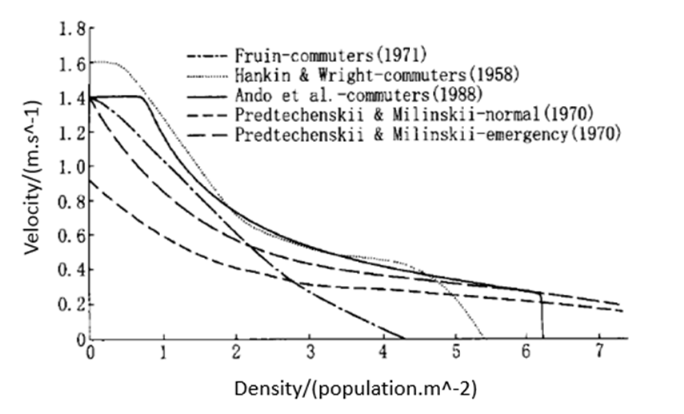
\includegraphics[scale=0.6]{figure6.png}
	\caption{Relationship between flow density and moving velocity}
	\label{fig:fig1}
\end{figure}

Based on the above study, Nelson and other researchers reached to 
a conclusion that when the population density is less than 0.54 people per 
$m^2$, people can move freely inside the experimental space. However, 
individuals will find difficultly in free movement under the circumstance 
of the population density is more than 3.8 people /$m^2$.\cite{8} Thus 
we can conclude that in the broad area like the hall and exhibition rooms, 
visitors can move freely without being affected by the people around them. 
From the Figure \ref{fig:fig1} above, we can set visitors' walking speed 
in these areas to a reasonable and stable value. (e.g. Set v$_{1}$=1.6m/s)

Actually, in some places where the movement area is narrow such as doors, 
stairs and elevators ,  the crowd flow density is relatively high, and 
individuals' movement is restricted and confined by the people around 
them that is to say that the evacuation speed of visitors is influenced 
by the crowd density.

There is an empirical formula between the speed of movement and the density of visitors based on the study from Koichi Kimura

\begin{equation}
    v_{2}=1.1\rho^{-0.7954}   
\end{equation}

The unit of  v$_{2}$  is $m/s$ and the unit of $\rho$ is $population/m^2$.

We utilized the Matlab drawing tool to draw its function graphics shown at the Figure \ref{fig:fig2} below.


\begin{figure}[htb] 
	\centering
	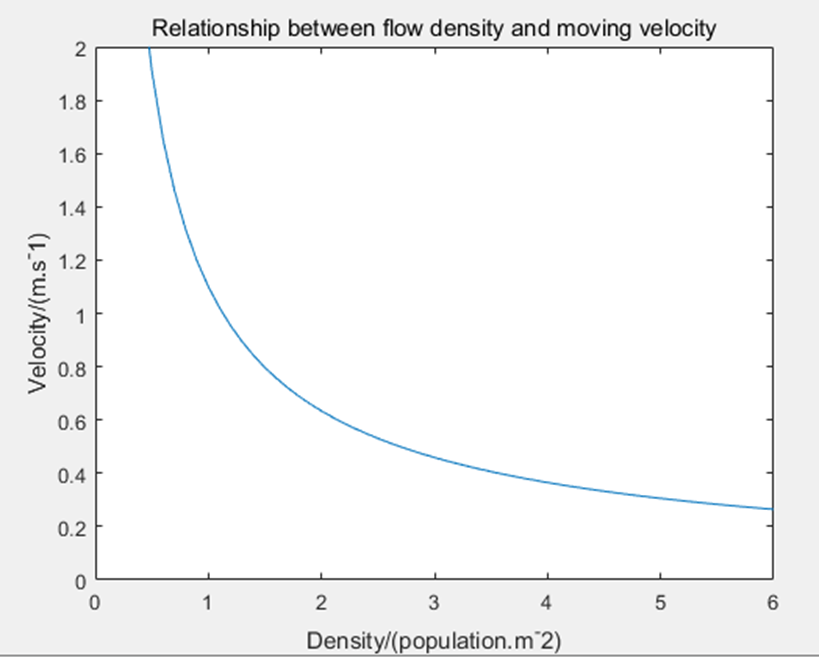
\includegraphics[scale=0.9]{figure7.png}
	\caption{Relationship between flow density and moving velocity}
	\label{fig:fig2}
\end{figure}

As can be seen from the graph, the results calculated 
by this formula coincides greatly with the observation results of Fruin ,
 Maclennan\&Nelson from America and Smith from the United Kingdom. 
 In essence, we could come to the conclusion that these two formulas are better coincident with each other 
 when the crowd flow density is between 1 $p/m^2$ and 5 $p/m^2$ based on the results of the graph. 
 (To simplify writing, the unit of the Density is all called $p/m^2$ for short.)

By means of the connection between the crowd flow density and move velocity, we can calculate the throughput of the visitors' evacuation in narrow places.

\begin{equation}
    T=\rho*v_{2}*w
\end{equation}

Here we represent the density of people in terms of two linear densities, which can be named as  the horizontal and vertical linear density.

The vertical linear density of the visitors is the number of people per unit length in their front and rear direction. Similarly, the horizontal linear density of the visitors is the number of people per unit length in their right and left direction.\cite{14} Hence, we can conclude the formula below:
\begin{equation}
    \rho=\rho_{1} * \rho_{2}  
\end{equation}

According to the data on fire safety principles of buildings in the former Soviet union compiled by M .Y .Roytman\cite{11}, the body thickness of adults in the front and rear directions is about 0.32 meter, and the body width on both sides is 0.5 meter under normal circumstances.

Considering the necessities to make the visitors get out of the danger zone as quickly as possible, we assume the contact density is the highest between visitors in the queue, which is to say we ignore the distance between individuals. Thus we can calculate the following results:

\begin{center}
$\rho_1=3(p/m^2)$  \\ 
$\rho_2=2(p/m^2)$   \\
$\rho=\rho_1*\rho_2=6(p/m^2)$
\end{center}

Based on the mathematical results, the throughput can be expressed as a 
function of the channels' effective width. The calculation formula is as follows:

\begin{equation}
    T=\rho*v_{2}*w=\rho*1.1*\rho^{-0.7954}*w=1.5871*w 
\end{equation}

Therefore when the crow flow density is high, these narrow spaces are very likely to become the potential bottlenecks which can be named as Potential Bottleneck Candidates(PBC). And, we utilize their throughput to evaluate their ability to influence evacuation time and then discover the actual potential bottlenecks among them.

\subsubsection{Modeling Process}

Through the discussion and analysis above,our team came to the conclusion that 
the visitors can be regarded as moving at a constant speed in the spacious places and as for the PBC place,the thoughput can reflect its congestion degree.

Therefore we altered the Weighted-Graph, endowing its vertices with  
weight as our new Graph Model. Thus we could utilize the weight edge of the graph to show the movement 
of visitors at spacious part of building and utilize the weight vertex of the graph to show PBC's situation(See Figure \ref{fig:fig3} and Figure \ref{fig:fig4}).

\begin{figure}[htb] 
	\centering
	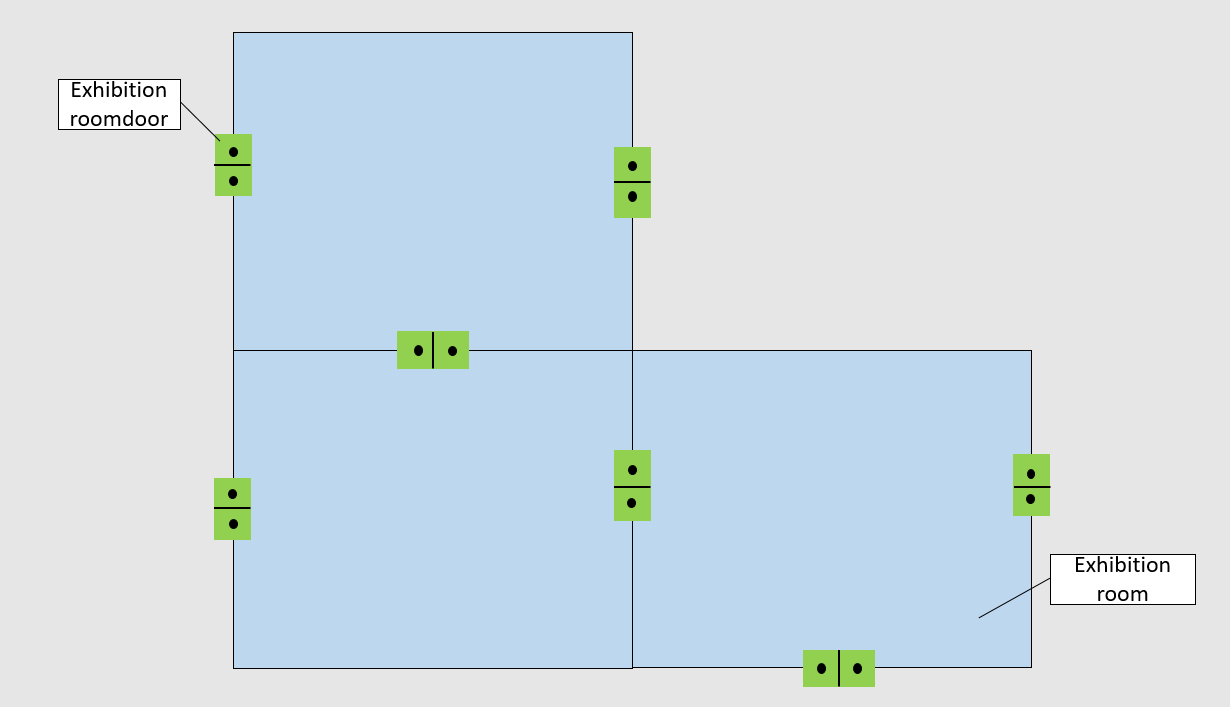
\includegraphics[scale=0.23]{figure4.png}
	\caption{An exhibition room before abstraction}
	\label{fig:fig3}
\end{figure}

\begin{figure}[htb] 
	\centering
	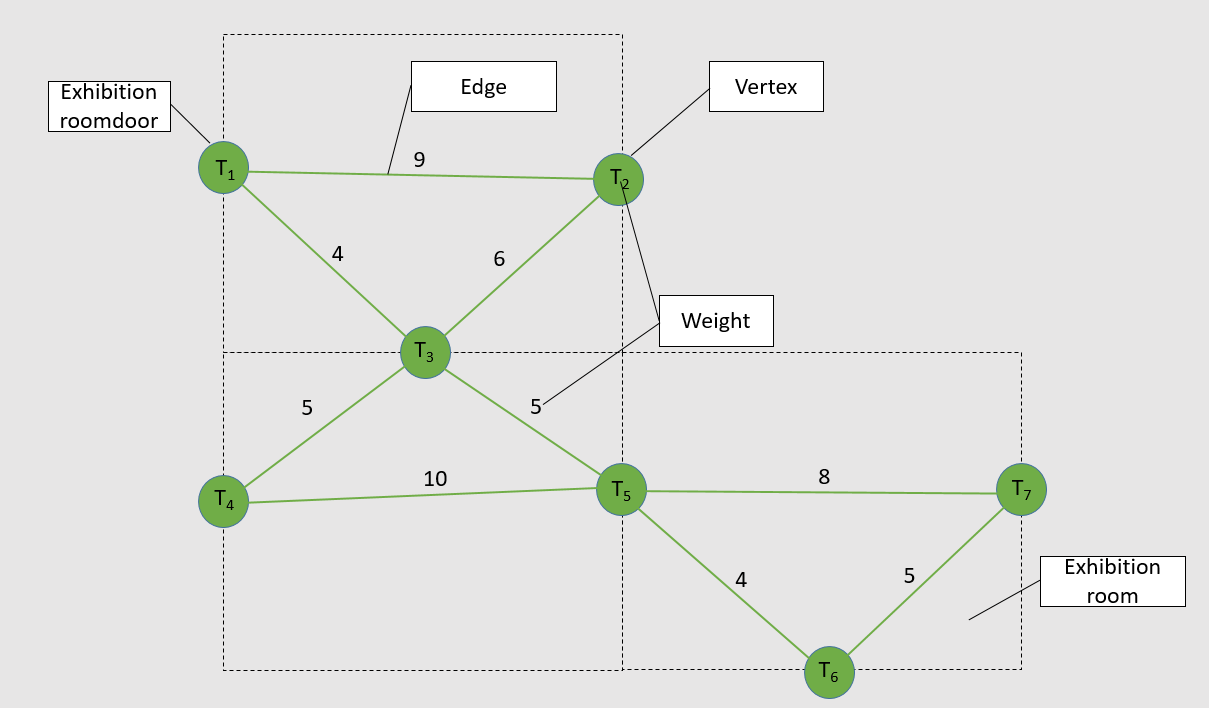
\includegraphics[scale=0.23]{figure5.png}
	\caption{An exhibition room after abstraction}
	\label{fig:fig4}
\end{figure}


Considering the crowd moving speed is constant, this method is actually 
efficient. We only need to measure the real distance between PBCs to obtain edges' weight values.
Meanwhile,we use PBC's thoughput as its weight which clearly and intuitively represent the congestion degree in narrow spaces at every moment.
We sorted the max-weight of all the vertices in descending order in order to compare the crowding degree of vertices, for the filtration of the potential bottlenecks(PB).




Due to the diversity of the actual situation, we suggest that the precise calculation of the crowded degree should be carried out after the PBC are confirmed as PB.
If only for the determination of the PB, the results needn't to be excessively accurate. You can utilize modern technology to gain more accurate results, when already selected out the PB.(See Section \ref{section:6})


We applied our model to the Louvre,and refined the PBC's type as follow:

\begin{figure}[htb]
	\centering
	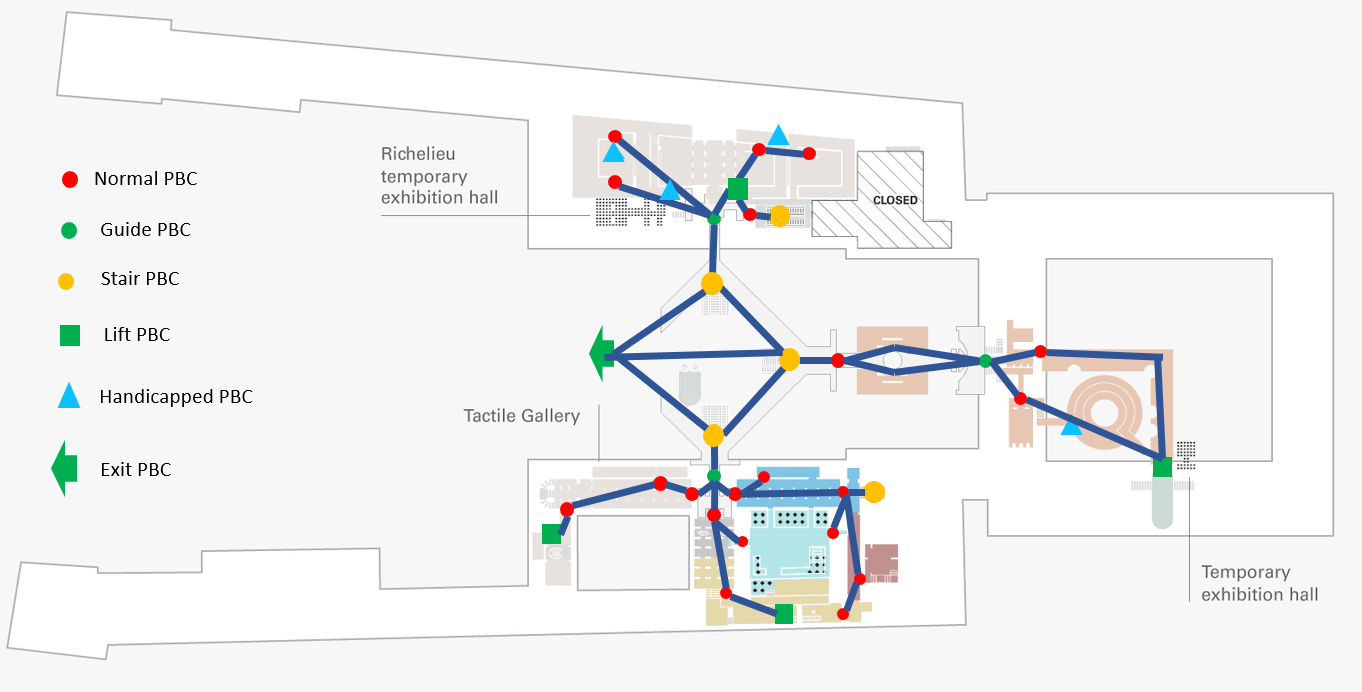
\includegraphics[scale=0.3]{figure1.png}
	\caption{Abstraction process of a floor of the Louvre.}
	\label{fig:fig5}
\end{figure}
\begin{figure}[htb]
	\centering
	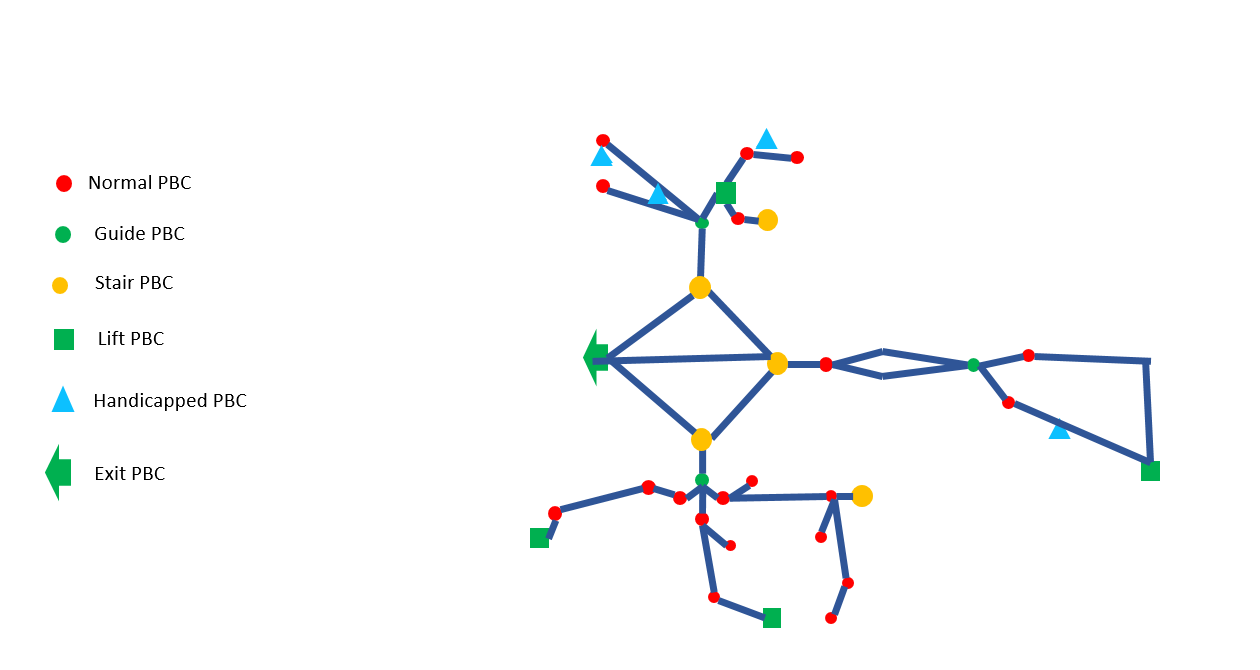
\includegraphics[scale=0.3]{figure2.png}
	\caption{Our abstraction graph model of the floor.}
	\label{fig:fig6}
\end{figure}



Normal PBC is similar to doors, stairs as well as narrow spaces which have the potential to bring congestion and jam.

Exit PBC represent the PBC which can let visitors finally exit the building.

Stair PBC can be used for floor changing. (See Section \ref{section:3.1.4})

Guide PBC means that this kind of PBC is equipped with 
the emergency personnel who are capable of providing the
 visitors with official guidance.(See Section \ref{section:3.1.5})

Handicapped PBC refer to the PBC designed for visitors wit disability or special needs.(See Section \ref{section:3.2.2})


Simultaneously,we use the moving point cluster on the graph to simulate 
the movement of visitors.By means of the Cellular Automata(CA) model,we set moving rule(See \ref{section:3.1.5}) to all the visitor point.Visitors point can automatically move towards the set exits based on the moving rule.Our team carried out the simulation of the entire process of the visitors' evacuation with or without the staff's guidance under the emergency situations,meanwhile we have the ability to capture the congestion degree of every PBC at every moment.
It is visualized and unambiguous for the model users or say the museum officials to consider the bottlenecks issue. In addition, this solution makes it easier to gather the information about when and how to utilize the AE and the entering plan for the emergency personnel.

\begin{figure}[h]
	\centering
	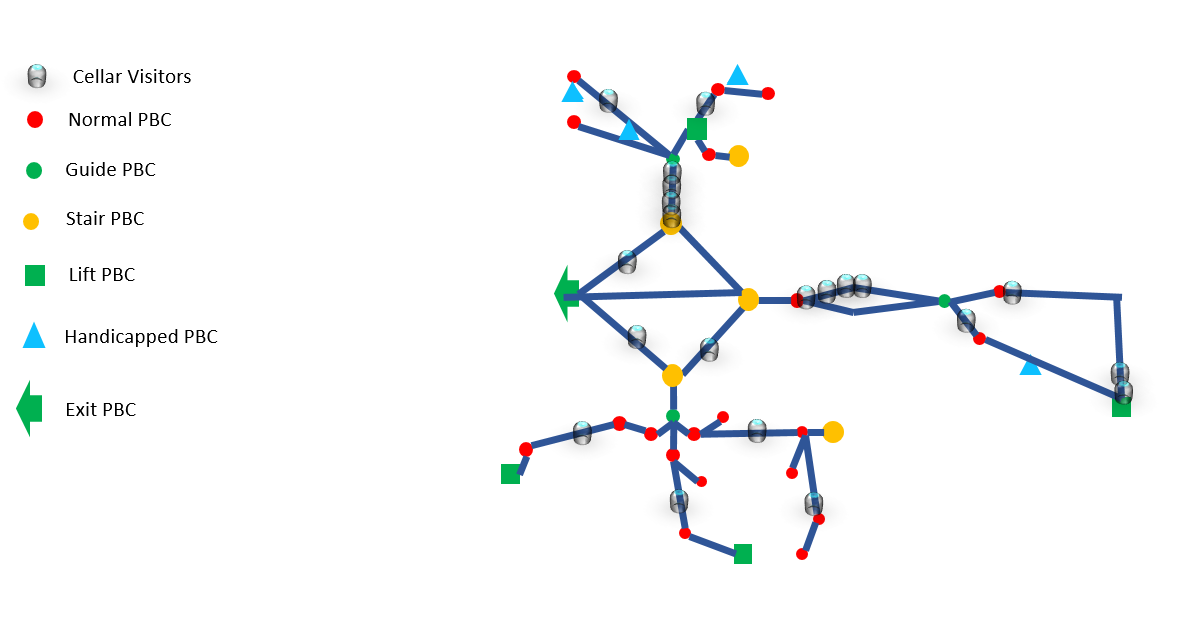
\includegraphics[scale=0.3]{figure3.png}
	\caption{Our graph model with visitor points on it.}
	\label{fig:fig7}
\end{figure}


\subsubsection{"Topple" High Building} \label{section:3.1.4}

Subsequently, we considered the three-dimensional characteristic of the building. 
Taking the Louvre as an example, we found that it is unworthy to individually consider each and every floor of the Louvre. This operation is of no actual significance and complicates the situation.
Moreover, we found that the staircase connects the two floors can
actually still be able to be regarded as a Nomal PBC. They can also be described by Nomal PBC's parameters such as congestion degree,connected vertices.



You can see that the influence to PBC caused by the different heights is nothing but distance to exits or availability,which Normal PBC has already been able to describe.
Thus, our team creatively abstracted the complex three-dimensional model into a big two-dimensional planar graph consist of the 
weighted edges and the weighted vertices. 
However, we still left the adequate adaptive adjustment space for the model using Stair PBC,you can change its height parameter,and use it
to decide whether take some extra measures about evacuation.



\subsubsection{The Simulation of Visitors' Movement} \label{section:3.1.5}
Many simulation models about the individual's movement issue under emergency 
have been established around the world at present, such as the early 
velocity-density model\cite{15}, the EVACNET model developed by the University 
of Florida\cite{16} and other macro models,also the SocialForce model by D.Helbing\cite{17} and other micro models. With 
the development of the computer technology, the calculating ability is no 
longer a constraint factor, thus the micro model which reflects the individual 
differences will be the mainstream of the emergency evacuation plan's future.    

Thus, to combine macro and micro model's advantages together, 
we hope to gain fundamental principle such as the queuing theory 
of PBC with the help of the macro model 
and use cellular automata(CA) as a micro model to simulate visitors' 
movement in reality.  

We also find that proper guidance from the emergency personnel is 
significantly important for the evacuation process\cite{13}. 
And the visitors are more likely to follow the instructions due to 
crowd psychology in panic which greatly increases the evacuation 
efficiency. Hence we also chose to add Guide PBC as vertex's type 
to simulate the route with the staff's guidance.

The moving rule we set for visitors and visitors under staff's guidance are shown in the table below:

\renewcommand\arraystretch{1.5}
\begin{tabular}{p{17em}|p{17em}}
    \hline
    \multicolumn{2}{c}{\textbf{\large{Cellular Rule}}} \\ \hline
	\textbf{Visitor} & \textbf{Visitor in Guide PBC} \\ \hline
1.Calculate the distance with edge weight from itself to all the Exit PBC, and choose the nearest to escape. & 1.	Calculate the distance with edge weight and \textbf{vertex weight} from itself to all the Exit PBC, and choose the nearest to escape. \textbf{Considering available AE as an Exit PBC also.} \\ \hline
2.Use Floyd-Warshall algorithm to find the shortest path to the Exit PBC. & 2.	Use Floyd-Warshall algorithm with \textbf{vertex weight} to update the shortest path to the Exit PBC. \\ \hline
3.Set people's speed at different $v_{0}$ to simulate visitor diversity. Start moving following the shortest path. & 3.Set people's speed at different $v_{0}$ to simulate visitor diversity. 	Start moving following the shortest path. \\ \hline
4.In the edge, move at $v_{0}$.In the vertex, if empty, go through; if crowd, queue up. & 4.	In the edge, move at $v_{0}$.In the vertex, if empty, go through; if crowd, queue up. \\ \hline
5.When arriving at Exit PBC, manage to escape. & 5. When arriving at Exit PBC, manage to escape. \\ \hline
\end{tabular}

Our model's strong adaptation allows its users to add new Guide PBC at any time to simulate the increase of staff number. Also, the model reserves the space for utilizing the clustering algorithm such as ant colony optimization(AOC) and particle swarm optimization(PSO) for the optimization.

\subsection{Model Optimization}
\subsubsection{Additional Exits(AE)}
Taking order and administration cost into consideration, our 
recommendation towards the Louvre is to close all the AE in 
advance and allow no private use of AE from any visitors. Only 
under the permission of the emergency personnel or the museum's 
official can some of the AE be used as the evacuation exit. 
Otherwise, neither the destruction of the museum's collections nor 
the potential dangers to the visitors is under control. 


Actually, the considerations of controllability 
should be given the highest priority when emergency happens.\cite{19}
We carried out the following discussion and analyses based on the controll abilitys' priority .

So,the question is: when and how to utilize additional exits?

Firstly, we addressed the issue about when to utilize AE.
With regard to the emergency personnel, we assume the emergency 
personnel is of the completed controllability and have a high level of urgency. 
As a consequence, all the AE should be
available to the emergency personnel unconditionally.
However for the visitors, our team believe that it actually an issue 
of the balance between safety and evacuation speed. When the evacuation 
speed can't ensure the visitors to evacuate before the detrimental emergency 
influence spread, we should give priority to the speed.
When there is no strict requirement of the evacuation time, the 
availability of AE should be avoided as it possibly can. We mainly 
take the following factors into consideration.
\begin{itemize}
    \item \textbf{The emergent degree}:To evaluate the urgency of the emergency.
    \item \textbf{Crowd flow density near the AE}:To reflect the congestion in this area.
    \item \textbf{Crowd flow density throughout the whole building}:To reflect the overall evacuation progress.
    \item \textbf{Safety}:The usage of AE could be a safety hazard due to the lack of security or to say the staff's guide.
\end{itemize}

Among this, the crowd flow density near the AE is the most intuitional determinant of whether to open it or not. And on this basis we also added the overall crowd flow density in the hope that in very urgent emergencies, opening AE to empty the visitors nearby can slightly relieve the congestion degree all the building.


We use the mathematical expression below as a judgment indicator. 

\begin{equation}
	K_{1}*m_{1}+K_{2}*m_{2}+K_{3}>\varepsilon  \label{pythagorean}
\end{equation}
	
Where $m_{1}$ indicates the crowd flow density near an AE, and
$m_{2}$ indicates the crowd flow density in the whole building.$K_{1}$ indicates the weight of $m_{1}$'s influence on our model.
$K_{2}$ indicates the weight of $m_{2}$'s influence on our model. 
$K_{3}$ indicates the influence 
caused by the emergent degree and safety.
When the ratio is greater than a certain threshold,
the AE can be put into use during evacuation.

Considering that the emergency degree of potential threats can only be determined upon the official's discussion and different AE have different safety performance, it is unlikely to find out the exact values of $K_{1}$, $K_{2}$ and $K_{3}$ with universality. Hence we only performed qualitative analysis of AE in this section. And we hope that our model users can take full account of the four factors we have listed above before determine the threshold value of AE. 

Secondly, about how to utilize AE, we stipulate that only with the guidance of the museum staff can visitors reach the particular AE. Simultaneously, we suggest to optimize the exit mode of AE in advance for safety assurances by more intelligent security detection.

Due to the assumption that all the visitors is forbid from the private 
and unreported use of the AE and most of the visitors don't know the 
exact location of the AE, the AE are represented by the unavailable 
vertices which means that the adjacency matrix value between he AE 
and other nodes is $\infty$ , so as to simulate the exits' closures. 
Also when an AE is available to the visitors, the adjacency matrix of 
the Guide PBC will be updated and simultaneously, the weight value is 
updated to the Edge which is directly connected with the available AE. 
And a new Guide PBC which in charge of this AE will be 
added to the graph in order to stimulate the opening up process 
of the AE after the staff receive the corresponding instruction. 
Thus the visitors are capable of evacuate the building safely 
and quickly with the guidance of the optimal evacuation route 
from the adjacency matrix value calculated by the Guide PBC.

\subsubsection{Visitors' Diversity} \label{section:3.2.2}

The Louvre as an international popular museum draws hundred of visitors around the world every day. Thus the diversity of the visitors is a very important aspect during the modeling process. The high diversity brought by different physical ability, speaking a variety of languages and visitor's complicated mental states makes our work more challenging. In the following paragraphs, we respectively analyzed the possible reasons of all the four differences and operable solutions to overcome the challenges.



\begin{enumerate}
	

\item Physical ability.The physical ability's differences among 
visitors are closely related to age, healthy condition and other factors. 
We suggest to set exclusive channels for visitors with mobility difficulties(the Louvre already has), 
such as infants, elderly people and people with disabilities in order 
to avoid the possible congestion. Handicapped PBC is added as the special channel
for visitors with mobility difficulties in our model.

\item Language.The diversity of the visitors' languages also provides challenge to our modeling process. According to official statistics, we summarized the proportion of the language spoken by the visitors as shown in the graph below.\cite{12}

\renewcommand\arraystretch{1.8}
\begin{tabular}{|c|c|c|c|c|c|c|}
    \hline
    German & Spanish & French & English & Chinese & Portuguese & Others \\
    \hline
    2.9\% & 2.7\% & 30\% & 16.4\% & 8\% & 3.5\% & 36.5\% \\
    \hline
\end{tabular}


Based on the data, we could work out the order of languages used for 
emergency broadcasting. And the individual audio guide which speaks the same language as the visitor can also be used for evacuation guidance at the first time. 

\item Mental state.It is barely possible to predict every individual's reaction 
towards the emergency. And the mental states of the visitors are also very 
complex. To deal with this issue, we could increase the number of the staff 
which is to add more Guide PBC.The staff's management can effectively ease the situation\cite{13}

\end{enumerate}

\subsubsection{Potential Threats and Emergency Personnel}
There are many potential threats during the process of the evacuation. 
The elevator may not work properly in case of fire, some particular 
routes are unavailable because of terrorists' occupy and the collapse 
caused by earthquake.These may bring new formidable challenges to the emergency 
management. 

Our model is highly adaptable and each of the potential threats is capable of adjust the existing optimal route to safety. Some typical examples are as follows:The vertices which represent elevators can be set to closed state in fire.The edges which represent temporarily occupied routes can be set to unavailable in terror attack. 
In this way, our model can still quickly make different optimal evacuation routes in many potential threats. And for the location of emergency, we can close the vertices and edges nearby and meanwhile increase the unavailable area close-by to simulate the emergency's diffusion.

We believe that once emergency happens, the immediate notification to emergency personnel is of the most importance. This can be accomplished by analyzing different weights in our model. Also to let them enter as quick as possible without adversely affect evacuation, the exclusive AE can be made available to them. And these exclusive AE for emergency personnel should be near the dangerous area to increase the evacuation's efficiency. 


\section{Experiment}
We use Java to complete our model. First we represented our model's function through simplified evacuation route and then we stimulated the evacuation process of the Louvre.(See appendix for source code and test data.)
\subsection{Model Validation}
In our simplified model, we firstly tested the evacuation process 
without Guide PBC or AE. The whole evacuation process takes 28 seconds, 
and at the 8th second, in the two nodes closest to the exit, no.1 and no.3, 
only the relatively near exit no.1 was congested with a large number of 
visitors, whereas node no.3 is not in use by any visitors. 
The running moment at 8th second are shown in the Figure \ref{fig:fig8}.
\begin{figure}[ht]
	\centering
	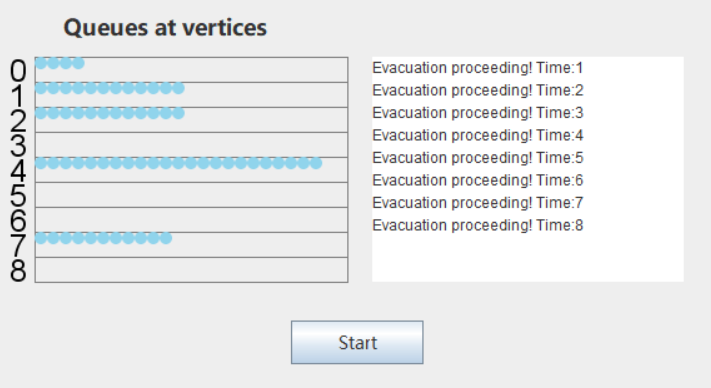
\includegraphics[scale=0.4]{figure9.png}
	\caption{Runing without Guide PBC.}
	\label{fig:fig8}
\end{figure}

When we use node no.4 as a Guide PBC and real-timely analyze the congestion condition, 
you can see that at the 8th second, if the staff can guide 
some visitors to the node no.3 for evacuation which ease the pressure of node no.1,
the total evacuation time can be reduced to 23s. Our model's advantage on 
increasing the evacuation's speed is legible and apparent. 

\begin{figure}[ht]
	\centering
	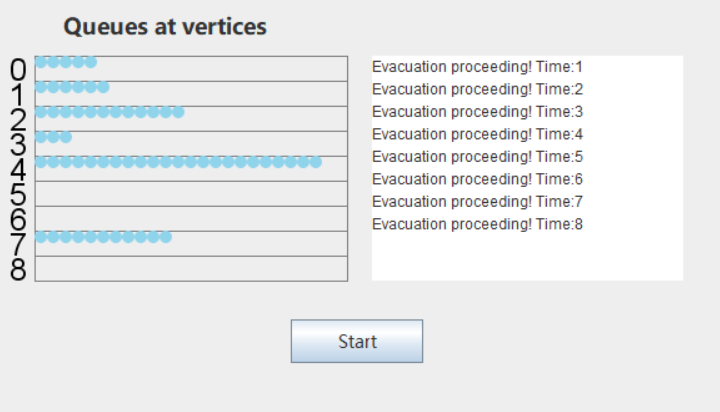
\includegraphics[scale=0.4]{figure10.png}
	\caption{Running with Guide PBC.}
	\label{fig:fig9}
\end{figure}

Then we added more AE into the test and set a threshold value for the congestion degree of AE.When the congestion degree reaches the threshold, the node no.9 should be made available to the visitors to ease the congestion. And the final evacuation time is 19 seconds.  

In our experiment, the graphical user interface(GUI) can 
provide real-time updates on the congestion degree of every PBC. Through this way, we can intuitively figure out potential bottlenecks as we expected.
\subsection{Implement to the Louvre}
Due to the lack of accurate drawings from the authorities, and it is difficult 
for us to make on-the-spot measurements. So our data can not be completely 
accurate. But based on the existing statistics, we made the maximized 
reproduction of the scene. We got the building structure through multiple versions of the museum's 
overview diagrams and detailed analyses of the three-dimensional building 
structures on Google Earth.And we gathered the latest visitors number in 2018 
and calculated the average daily number of visitors. We manually selected out
PBCs and put this data into our model, then we 
gained the results as follows:

\begin{figure}[ht]
	\centering
	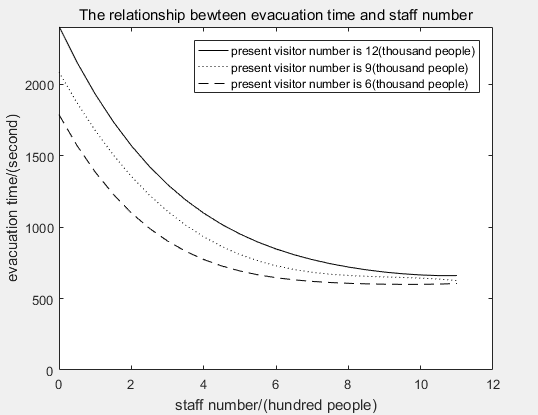
\includegraphics[scale=0.8]{figure11.png}
	\caption{The relationship between evacuation time and staff number.}
	\label{fig:fig10}
\end{figure}

\begin{figure}[ht]
	\centering
	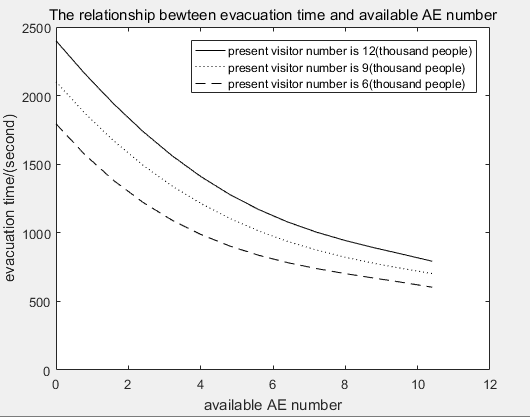
\includegraphics[scale=0.8]{figure12.png}
	\caption{The relationship between evacuation time and available AE number.}
	\label{fig:fig11}
\end{figure}


But with field survey, multiple experiments and abundant manpower and material 
resources, theoretically we could get optimal evacuation route.

\subsection{Sensitivity Analyses}
We simultaneously analyzed three sets of data in pairs which are visitor number, staff number and available AE number. The results are shown in the Figure \ref{fig:fig10} and Figure \ref{fig:fig11}.

From the results,we concluded that staff number and available AE number have more significant influence on the total evacuation time when the present visitor number is larger. And when staff number and available AE number increase, evacuation time's decrease range will be larger. This indicates that for large and crowed buildings like the Louvre, it is of huge significance for the emergency evacuation to add more exits and provide more guidance. 
And when the present visitor number is small, there are few constraints to people's movement, thus the evacuation time will be quite short. This indicates that we should limit visitor number to a reasonable and appropriate range.


\subsection{Implement to other large, crowded structures}

For other large, crowded structures, we could also select narrow spaces as PBC, measure  their effective width, and then calculate their throughput to gain weight of edge and vertices. Aimed at different present visitor number, we could utilize our cellular rule, test and search potential bottlenecks and accomplish real-time monitoring for each potential bottleneck to timely divert visitors. Also through the stimulated threshold value of AE, we could estimate whether to open more AE or not. Furthermore, to gain the optimal evacuation plan, we could timely update the graph's structure on the basis of the real-time situation. 


Our recommendations for the emergency management of the Louvre are also adaptable to other large buildings. 



\section{Strengths and Weaknesses}
\subsection{Strengths}
\begin{itemize}
	\item \textbf{We combined the advantages of cellular 
	 and graph theory.}
	
	The cellular automata can subtly simulate human behavior, but it doesn't give an intuitive sense of what's going on in the environment, while Graph theory is just the opposite.We greatly improved the adaptability of our model by combining their advantages and avoiding their shortcoming, so that our model can reflect and solve various types of potential threats whatever to human or the structure.
	
	\item \textbf{We creatively abstracted the three-dimensional model into a big two-dimensional planar graph.}
	
	By doing this, we ignored the unnecessary factors, and our model's efficiency is increased to a great extent consequently. Simultaneously, it is clearer and more intuitionistic when it comes to the analyses of our model.  
	
	
	\item \textbf{We analyzed visitor's movement both in micro level and macro level.}
	
	In the microscopical layer, we regard the visitors as fluid by 
	utilizing the density-velocity model. In the macroscopical layer, 
	we regard visitor's movement as cellular's movement by utilizing 
	the cellular automata(CA) model. Microscopic method was designed 
	for the actual calculations, while macroscopic method was 
	designed for the theoretical analyses.  
	
\end{itemize}

\subsection{Weaknesses}
\begin{itemize}
	\item \textbf{Some data inaccuracy.}
	Because plenty of the relative data is unavailable on the Internet or the other information platform, our team could only utilize the existing data,which may cause some deviation.
	
	\item \textbf{Some partial considerations.}
	Our model focuses on adaptability, so some of the more subtle problems are not fully realized, such as the simulation of human herd psychology.We hope that in future work, we can use cluster optimization to continue to improve.
	 
	
 \end{itemize}



\section{Recommendations for the Louvre} \label{section:6}
We were asked to propose policy and procedural recommendations in our paper. Therefore, our team discussed and proposed several feasible proposals on how to evacuate visitors as quick and safe as possible for the emergency management of the Louver based on the results and statistics of our model.
\begin{enumerate}
\item \textbf{Limit the maximum number of the visitors inside the Louvre.} 

From the experiment results, we concluded that the evacuation process takes more time when the number of visitors is larger. Therefore, it would be much better if the Louvre can limit the number of the visitors to an appropriate level. Meanwhile, the Affluences app had better not to only show the estimated waiting time, but also show the real-time number of present visitors to offer advice on whether to visit the Louvre or not.


\item \textbf{Utilize apps designed respectively for visitors and the museum staff below.}

The app for visitors should be capable of supporting multiple languages, providing clear information about the available AE and optimal evacuation route. 
The app for staff should provide real-time interaction of information about the congestion degree of potential bottlenecks and availability of AE to enhance their assistant ability.
  
\item \textbf{Make more use of modern technology.} 

Utilize machine learning and other intelligence technologies to estimate the congestion degree of PB, discover the bottlenecks in time and react accordingly. Issue in-time alarming of the potential danger to prevent stampede and other accidents from happening. 

\item \textbf{Establish connection with government in advance.}

This enables the Louvre to get professional help at the first time from emergency personnel of the nearby fair stations, hospitals and the police stations.  

\end{enumerate}


\begin{thebibliography}{99}
\addcontentsline{toc}{section}{References}  %引用部分标题("Refenrence")的重命名


\bibitem{1}CNBC,DAVOS WORLD ECONOMIC FORUM: Silvia Amaro, A pessimistic population means Yellow Vest protests 
could become more mainstream, new survey warns.2018.01.23.\\ \url{https://www.cnbc.com/2019/01/21
/frances-yellow-vest-protests-could-become-more-mainstream-survey-warns.html}


\bibitem{2}Tencent Website: The number of visitors to the Louvre in France exceeded 10 million in 2018.2019.01.04.\\ \url{https://
new.qq.com/omn/20190104/20190104A0239N.html}

\bibitem{3}LIU BEI, MIU YALI, The Louvre re-emerges as the most visited museum in the world. \emph{Art Museum Magazine},2018.07.16.\\ \url{https://
js.ifeng.com/a/20180716/6729002_0.shtml}




\bibitem{7}PREDTECHENSKII V M, MILINSKI A I .Planning for foot traffic flow in building 
               [M] .Stroiizdat Publishers,Moscow,1969.

\bibitem{8}PHILIT J D, CRAIG J D, RICHARD L R, et al.SFPE Handbook of Fire Protection Engineering[S] .Published by National fire protection association , 1995 .

\bibitem{9}SMITH R A.Density , velocity and flow relationships for closely packed
               crowds[J].Safety Science, 1995, 18 :321-327 .

\bibitem{10}THOMPSON P A, MARCHANT E W.Computer and fluid modelling of evacuation[J] .Safety Science , 1995, 18:277-289.

\bibitem{11}ROYTMAN, M Y.Principles of fire safety standards for building construction[M]. Amerind publishing Co .New Delhi,1975 .

\bibitem{12}“8.1 Million Visitors to the Louvre in 2017.” \emph{Louvre Press Release}, 25 Jan. 2018,\\\url{presse.louvre.fr/8-1-million-visitors-to-the-louvre-in-2017/}.

\bibitem{13}LI Qiang, CUI Xihong, CHEN Jin. Study on occupant evacuation process from large public facilities and effect of guidance. \emph{JOURNAL OF NATURAL DISASTERS}, 2006

\bibitem{14}HUANG XIFA, WANG KEJUN,ZHANG LEI, WANG YING, Study on a microscopic model of pedestrian evacuation based on different individual capacity. 
\emph{Journal of Safety Science and Technology}, 2009.10

\bibitem{15}
G.Keith Still, Crowd Dynamics, \emph{PhD Thesis}, University of Warwick, 2000

\bibitem{16}
T.Kisko, R.Francis and C.Noble, \emph{EVACENET 4 User's Guide},[R], University of Florida, 1998

\bibitem{17}
D.Helbing, SocialForce model for pedestrian dynamics,  \emph{Physical Review E}, 1995 51(5):
4288~4268

\bibitem{19}CHENG Yuan. \emph{Research on Crowd Evacuation Behaviors Baesd on Evolutionary Game Theory}, Page6, 2012

\bibitem{18}LU Jun-an, FANG Zheng, LO Siu-ming, ZHAO Chun-mei. \emph{Mathematical model of evacuation speed for personnel in buildings}, 2002. Engineering Journal of Wuhan University.

\end{thebibliography}


% ==============以下为附录内容,如您的论文中不需要程序附录请自行删除====================
\clearpage
\begin{subappendices}						% 附录环境
\section*{Apendix: The source codes and test data}		% 附录标题可以自行修改
\addcontentsline{toc}{section}{Appendix}  	% 将附录内容加入到目录中

The adjacent matrix for testing the Louvre (M means $\infty$) :\\
\\
\small{
{0,M,M,M,M,M,M,M,M,M,M,M,M,M,M,M,M,M,M,M,M,400,M,M,M,M,M,M,M,M,M,M,M}\\
{M,0,150,M,M,M,M,M,M,M,M,M,M,M,M,M,M,M,M,M,150,M,M,M,M,M,M,M,M,M,M,M,M}\\
{M,150,0,M,M,M,M,M,M,M,M,M,M,M,M,M,M,M,M,M,M,M,M,M,M,M,M,M,M,M,M,M,M}\\
{M,M,M,0,M,M,M,M,M,M,M,M,M,M,M,M,M,M,M,M,M,300,M,M,M,M,M,M,M,M,M,M,M}\\
{M,M,M,M,0,M,M,M,M,M,M,M,M,M,M,M,M,M,M,M,50,M,M,M,M,M,M,M,50,M,M,M,M}\\
{M,M,M,M,M,0,M,M,M,M,M,M,M,M,M,M,M,M,M,M,M,M,M,450,M,M,M,M,M,M,100,M,M}\\
{M,M,M,M,M,M,0,M,M,M,M,M,M,M,M,M,M,M,M,M,M,M,M,150,600,M,M,M,M,M,M,M,M}\\
{M,M,M,M,M,M,M,0,M,M,M,M,M,M,M,M,M,M,M,M,M,M,M,150,500,M,M,M,M,M,M,M,M}\\
{M,M,M,M,M,M,M,M,0,300,M,M,M,M,M,M,M,M,M,M,M,M,M,M,M,M,50,M,M,M,M,M,M}\\
{M,M,M,M,M,M,M,M,300,0,100,M,M,M,M,M,M,M,M,M,M,M,M,M,M,M,M,M,M,M,M,M,M}\\
{M,M,M,M,M,M,M,M,M,100,0,M,M,M,M,M,M,M,M,M,M,M,M,M,M,50,M,M,M,M,M,M,M}\\
{M,M,M,M,M,M,M,M,M,M,M,0,100,400,M,M,M,M,M,M,M,M,M,M,M,50,M,M,M,M,M,M,M}\\
{M,M,M,M,M,M,M,M,M,M,M,100,0,M,M,M,M,M,M,M,M,M,M,M,M,M,M,M,M,M,M,M,M}\\
{M,M,M,M,M,M,M,M,M,M,M,400,M,0,M,100,M,250,M,M,M,M,M,M,M,M,M,M,M,M,M,M,50}\\
{M,M,M,M,M,M,M,M,M,M,M,M,M,M,0,M,150,M,250,M,M,M,M,M,M,150,M,M,M,M,M,M,M}\\
{M,M,M,M,M,M,M,M,M,M,M,M,M,100,M,0,M,M,M,M,M,M,M,M,M,M,M,M,M,M,M,M,M}\\
{M,M,M,M,M,M,M,M,M,M,M,M,M,M,150,M,0,M,M,M,M,M,M,M,M,M,M,M,M,M,M,M,M}\\
{M,M,M,M,M,M,M,M,M,M,M,M,M,250,M,M,M,0,M,150,M,M,M,M,M,M,M,M,M,M,M,M,M}\\
{M,M,M,M,M,M,M,M,M,M,M,M,M,M,250,M,M,M,0,M,M,M,M,M,M,M,M,200,M,M,M,M,M}\\
{M,M,M,M,M,M,M,M,M,M,M,M,M,M,M,M,M,150,M,0,M,M,M,M,M,M,M,M,M,M,M,M,M}\\
{M,150,M,M,50,M,M,M,M,M,M,M,M,M,M,M,M,M,M,M,0,50,M,M,M,M,M,M,M,M,M,M,M}\\
{400,M,M,300,M,M,M,M,M,M,M,M,M,M,M,M,M,M,M,M,50,0,M,M,M,M,M,M,M,200,M,M,M}\\
{M,M,M,M,M,M,M,M,M,M,M,M,M,M,M,M,M,M,M,M,M,M,0,M,M,M,M,M,M,400,500,450,M}\\
{M,M,M,M,M,450,150,150,M,M,M,M,M,M,M,M,M,M,M,M,M,M,M,0,M,M,M,M,M,M,M,M,M}\\
{M,M,M,M,M,M,600,500,M,M,M,M,M,M,M,M,M,M,M,M,M,M,M,M,0,M,M,M,M,M,M,M,M}\\
{M,M,M,M,M,M,M,M,M,M,50,50,M,M,150,M,M,M,M,M,M,M,M,M,M,0,M,M,M,M,M,100,M}\\
{M,M,M,M,M,M,M,M,50,M,M,M,M,M,M,M,M,M,M,M,M,M,M,M,M,M,0,M,M,M,M,M,M}\\
{M,M,M,M,M,M,M,M,M,M,M,M,M,M,M,M,M,M,200,M,M,M,M,M,M,M,M,0,M,M,M,M,M}\\
{M,M,M,M,50,M,M,M,M,M,M,M,M,M,M,M,M,M,M,M,M,M,M,M,M,M,M,M,0,M,M,M,M}\\
{M,M,M,M,M,M,M,M,M,M,M,M,M,M,M,M,M,M,M,M,M,200,400,M,M,M,M,M,M,0,350,M,M}\\
{M,M,M,M,M,100,M,M,M,M,M,M,M,M,M,M,M,M,M,M,M,M,500,M,M,M,M,M,M,350,0,300,M}\\
{M,M,M,M,M,M,M,M,M,M,M,M,M,M,M,M,M,M,M,M,M,M,450,M,M,100,M,M,M,M,300,0,M}\\
{M,M,M,M,M,M,M,M,M,M,M,M,M,50,M,M,M,M,M,M,M,M,M,M,M,M,M,M,M,M,M,M,0}\\
}


The weights of the vertices :\\
3.1742, 2.8568, 3.4916, 4,7613, 3.9678, 3.4916, 2.3806, 1.5871, 3.1742, 2.3806, 4.7613, \\
4.7613, 3.9678, 2.8568, 3.9678, 2.8568, 3.4916, 4.7613, 2.8568, 3.1742, 3.9678, 3.9678, \\
1.5871, 3.4916, 2.3806, 2.8568, 6.3484, 4.7613,3.1742, 4.7613,3.4916, 2.8568, 3.1742

Java program with demo test data :


\begin{lstlisting}[language=Java, caption=\texttt{Demo program}]
	import util.*;

import javax.swing.*;

import java.awt.*;
import java.awt.event.ActionEvent;
import java.awt.event.ActionListener;
import java.util.Timer;
import java.util.TimerTask;

public class main {
	

    public static void main(String[] args) {
    	

        EventQueue.invokeLater(new Runnable() {
            @Override
            public void run() {
    
                MyFrame frame = new MyFrame();
                frame.btnStart.setSize(106, 35);
                frame.textArea.setSize(249, 180);
                frame.btnStart.setFont(new Font("微软雅黑", Font.PLAIN, 14));
                frame.btnStart.setText("Start");
                frame.textArea.setLocation(300, 47);

                frame.btnStart.setLocation(235, 258);
                frame.p.setBounds(10, 47, 278, 201);
                
                JLabel lblQueuesAtVertices = new JLabel("Queues at vertices");
                lblQueuesAtVertices.setFont(new Font("微软雅黑", Font.BOLD, 18));
                lblQueuesAtVertices.setBounds(53, 10, 196, 27);
                frame.getContentPane().add(lblQueuesAtVertices);
                
     
                frame.setVisible(true);
            }
        });
        
    }


    public static class MyFrame extends JFrame  implements ActionListener{
    	static public Graph gra = new Graph();
        public static final String TITLE = "Queues at vertices";
        public static MyPanel p;
        public static final int WIDTH = 500;
        public static final int HEIGHT = 400;
        public JButton btnStart;
        public JTextArea textArea;
        Timer timer = null;
        int time = 0;
        public MyFrame() {
            super();
            initFrame();
            
            for(int i = 0;i<gra.VertxNum;i++) {
    			if(i ==0 ) {
    				gra.Vertex[i]=new ExitNode(i,8);
    				continue;
    			}
    			if(i == 4 ) {
    			gra.Vertex[i]=new GuideNode(i,3);
    			continue;
    			}
    			gra.Vertex[i]=new Node(i,3);
    		}
    		
    		
    		for(Node node:gra.Vertex) {
    			if(node.getClass()!=ExitNode.class) {
        		node.ini.add(new People(0,0,3,0,0,0,3));
        		node.ini.add(new People(0,0,3,0,0,0,3));
        		node.ini.add(new People(0,0,3,0,0,0,3));
        		node.ini.add(new People(0,0,3,0,0,0,3));
    			node.ini.add(new People(0,0,3,0,0,0,3));
    			node.ini.add(new People(0,0,3,0,0,0,3));
    			node.ini.add(new People(0,0,3,0,0,0,3));
    			node.ini.add(new People(0,0,3,0,0,0,3));
    			node.ini.add(new People(0,0,3,0,0,0,3));
    			node.ini.add(new People(0,0,3,0,0,0,3));
    			node.ini.add(new People(0,0,3,0,0,0,2));
    			node.ini.add(new People(0,0,3,0,0,0,2));
    			node.ini.add(new People(0,0,3,0,0,0,1));
    			node.ini.add(new People(0,0,3,0,0,0,1));


    			}
    		}
    		
            
        }

        private void initFrame() {

   
            setTitle(TITLE);
 
            setSize(WIDTH, HEIGHT);

            setDefaultCloseOperation(WindowConstants.EXIT_ON_CLOSE);
            
            setLocationRelativeTo(null);
            
            JPanel contentPane = new JPanel();
            contentPane.setLayout(null);
            setContentPane(contentPane);
            MyPanel panel = new MyPanel(this,gra);
            panel.setBounds(0, 0, 250, 230);
            contentPane.add(panel);
            p = panel;
           
            
            btnStart = new JButton("start");
    		btnStart.setBounds(190,230, 93, 23);
    		contentPane.add(btnStart);
    		btnStart.addActionListener(this);
    		
    		textArea = new JTextArea();
    		contentPane.add(textArea);
    		textArea.setBounds(260, 63, 200, 180);
    		
    	

            
        }
        
        public void startThread() {
    		if(timer!=null) {
    			timer.cancel();
    		
    		}
    		timer = new Timer();
    		timer.scheduleAtFixedRate(new MyTask(), 100, 1000);;
    		
    	}
        

    	public class MyTask extends TimerTask{

    		@Override
    		public void run() {
    			p.updateUI();
    			
    			
    			time ++;
    			Graph.oneSecondPassed(gra, 0);
    			for(int k = 0;k<gra.VertxNum;k++) {
    				gra.isTrav[k] = 0;
    			}
    			if(Graph.hasNoPeople(gra)) {
    				textArea.append("Evacuation success! Time:"+time+"\n");
    				
    			}
    			else {
    				textArea.append("Evacuation proceeding! Time:"+time+"\n");
    			}

    		}
    			
    	}
    
        @Override
		public void actionPerformed(ActionEvent e) {
        	if (e.getSource() == btnStart) {
        		startThread();
        		}
        	}
	
		}

    public static class MyPanel extends JPanel {

        private MyFrame frame;
        private Graph gra;

        public MyPanel(MyFrame frame,Graph gra) {
            super();
            this.frame = frame;
            this.gra = gra;
        }

        @Override
        protected void paintComponent(Graphics g) {
            super.paintComponent(g);

            drawRect(g);

             drawArc(g);

        }


        private void drawRect(Graphics g) {
            
            Graphics2D g2d = (Graphics2D) g.create();

			g2d.setRenderingHint(RenderingHints.KEY_ANTIALIASING, 
			RenderingHints.VALUE_ANTIALIAS_ON);
            g2d.setColor(Color.GRAY);

        
            for(int i=0;i<gra.VertxNum;i++) {
            	g2d.drawRect(20, i*20, 250, 20);
            }
            
            g2d.setColor(Color.BLACK);
            
            g2d.setFont(new Font(null, Font.PLAIN, 25));

            for(int i=0;i<gra.VertxNum;i++) {
            	g2d.drawString(new Integer(i).toString(), 0, i*20+20);
            }
            
           

            g2d.dispose();
        }

       
        private void drawArc(Graphics g) {
            
            Graphics2D g2d = (Graphics2D) g.create();

			g2d.setRenderingHint(RenderingHints.KEY_ANTIALIASING, 
			RenderingHints.VALUE_ANTIALIAS_ON);
            

            g2d.setColor(new Color(144, 212, 236));

            for(int i = 0;i<gra.VertxNum;i++) {
            	
            	if(gra.Vertex[i].que.isEmpty()==false) {
            	for(int t=0;t<gra.Vertex[i].que.size();t++)
            	{
            		g2d.fillArc(20+t*10, i*20, 10, 10, 90, 360);
            	}
            	}
            }

            g2d.dispose();
        }


    }
}



	package util;

	import java.util.ArrayList;
	import java.util.Iterator;
	import java.util.LinkedList;
	import java.util.List;
	import java.util.Queue;
	
	public class ExitNode extends Node {
	
		public ExitNode(int nodeId, int thoughPut) {
			super(nodeId, thoughPut);
			this. que = new LinkedList<>(); 
			this. ini = new ArrayList<>();
			this. peopleInEdge = new ArrayList<>();
		}
	
		@Override
		public void pass(Graph g) {
			
				for(int j=0;j<this.thoughPut;j++) {
					while(!this.que.isEmpty()) {
					this.que.poll();
					}
				}
			
		}
	
		@Override
		public void init(Graph g) {
			
		}
	
		@Override
		public void arrive(Graph g) {
			
		}
		
	}

	
	package util;

	import java.text.StringCharacterIterator;
	import java.util.ArrayList;
	
	import java.util.List;
	
	import javax.swing.text.StringContent;
	
	public class Graph {
		
	
	
		static final int MaxValue=65535;
		static final int M=65535;
		public Node[] Vertex = new Node[9];         
		
	 
		public int VertxNum = 9;              
		   
		
		int[][] EdgeWeight = {
				{0,4,6,2,M,M,M,M,M},
				{4,0,M,M,2,M,M,M,M},
				{6,M,0,M,M,M,M,3,M},
				{2,M,M,0,5,M,M,M,M},
				{M,2,M,5,0,3,3,M,M},
				{M,M,M,M,3,0,M,M,M},
				{M,M,M,M,3,M,0,M,M},
				{M,M,3,M,M,M,M,0,4},
				{M,M,M,M,M,M,M,4,0}
		};     
		public int[] isTrav = new int[9];            
		
		public static void oneSecondPassed(Graph g,int n){
			int i;
			g.isTrav[n] = 1;
			Node node = g.Vertex[n];
			
	
			node.pass(g);
			
	
			node.init(g);
			
	
			node.arrive(g);
			
			
			for(i = 0; i< g.VertxNum; i++)
			{
			
							if(g.EdgeWeight[n][i] != g.M && g.isTrav[i] == 0)
					{
							oneSecondPassed(g, i);     
					}
			}
		}
	
		public static boolean hasNoPeople(Graph g) {
			for(Node node:g.Vertex) {
				if(!node.ini.isEmpty()||!node.peopleInEdge.isEmpty()||
				!node.que.isEmpty()) {
					return false;
				}
			}
			
			return true;
		}
	
		public static int[] GetGuidePath(Graph g, int start, int exit,int speed) {
	
	
			int [] result = new int[100];
	
					
					int [][] pathMatirx = new int[g.VertxNum][g.VertxNum];
	
					int [][] preTable = new int[g.VertxNum][g.VertxNum];
					
					for (int i = 0; i < g.VertxNum; i++) {
						for (int j = 0; j < g.VertxNum; j++) {
							pathMatirx[i][j] = g.EdgeWeight[i][j]/speed
							+g.Vertex[j].que.size()/g.Vertex[j].thoughPut;
							preTable[i][j] = j;
						}
					}
	
					for (int k = 0; k < g.VertxNum; k++) {
	
						for (int m = 0; m < g.VertxNum; m++) {
							
							for (int n = 0; n < g.VertxNum; n++) {
								
								int mn = pathMatirx[m][n];
								int mk = pathMatirx[m][k];
								int kn = pathMatirx[k][n];
								int addedPath = (mk == M || kn == M)? M : mk + kn;
								
								if (mn > addedPath) {
	
									pathMatirx[m][n] = addedPath;
	
									preTable[m][n] = preTable[m][k];
								}
								
							}
						}
					}
					
					int k = preTable[start][exit];
					result[0] = start;
					int id = 1;
					while(k!=exit) {
						result[id] = k;
						id++;
						k = preTable[k][exit];
					}
					result[id] = exit;
					return result;
		}
		
		
		
		public static int[] GetShortestPath(Graph g, int start, int exit) {
	
			int [] result = new int[100];
	
		
			int [][] pathMatirx = new int[g.VertxNum][g.VertxNum];
	
			int [][] preTable = new int[g.VertxNum][g.VertxNum];
			
	
			for (int i = 0; i < g.VertxNum; i++) {
				for (int j = 0; j < g.VertxNum; j++) {
					pathMatirx[i][j] = g.EdgeWeight[i][j];
					preTable[i][j] = j;
				}
			}
			
	
			for (int k = 0; k < g.VertxNum; k++) {
	
				for (int m = 0; m < g.VertxNum; m++) {
					
					for (int n = 0; n < g.VertxNum; n++) {
						
						int mn = pathMatirx[m][n];
						int mk = pathMatirx[m][k];
						int kn = pathMatirx[k][n];
						int addedPath = (mk == M || kn == M)? M : mk + kn;
						
						if (mn > addedPath) {
	
							pathMatirx[m][n] = addedPath;
	
							preTable[m][n] = preTable[m][k];
						}
						
					}
				}
			}
			
			int k = preTable[start][exit];
			result[0] = start;
			int id = 1;
			while(k!=exit) {
				result[id] = k;
				id++;
				k = preTable[k][exit];
			}
			result[id] = exit;
			return result;
	
		}
		
	}
	

	package util;

	import java.util.ArrayList;
	import java.util.LinkedList;
	
	public class GuideNode extends Node {
			int exitnode;
		public GuideNode(int nodeId, int thoughPut) {
			super(nodeId, thoughPut);
			this. que = new LinkedList<>(); 
			this. ini = new ArrayList<>();
			this. peopleInEdge = new ArrayList<>();
			
		}
	
		@Override
		public void pass(Graph g) {
			for(int j=0;j<this.thoughPut;j++) {
				if(!this.que.isEmpty()) {
					People people = this.que.poll();
					people.escapePath = Graph.GetGuidePath(g,this.nodeId,
					this.exitnode,people.speed);
					people.position = 0;
					people.fromNode = this.nodeId;
					people.towardsNode = people.escapePath[people.position+1];
					people.walkTime = 
					g.EdgeWeight[people.fromNode][people.towardsNode];
					this.peopleInEdge.add(people);
				}
				
			}
		}
	
	
	}

	
	package util;


import java.util.ArrayList;
import java.util.Iterator;
import java.util.LinkedList;
import java.util.List;
import java.util.Queue;

public class Node {
	public Queue<People> que = new LinkedList<>(); 
	public List<People> ini = new ArrayList<>();
	public List<People> peopleInEdge = new ArrayList<>();
	public int nodeId = 0;
	
	public Node(int nodeId, int thoughPut) {
		super();
		this.nodeId = nodeId;
		this.thoughPut = thoughPut;
	}

	public int thoughPut = 2;
	
	public void pass(Graph g) {
		
			for(int j=0;j<this.thoughPut;j++) {
				if(!this.que.isEmpty()) {
					People people = this.que.poll();
					people.fromNode = this.nodeId;
					people.towardsNode = people.escapePath[people.position+1];
					people.walkTime = 
					g.EdgeWeight[people.fromNode][people.towardsNode];
					this.peopleInEdge.add(people);
				}
				
			}
	}

	public void arrive(Graph g) {
		for (Iterator<People> it = this.peopleInEdge.iterator(); it.hasNext();) {
			People item = it.next();
			if(item.walkTime!=0 ) {
				item.walkTime = item.walkTime - item.speed;
			}
			if(item.walkTime <= 0) {
				item.position++;
				g.Vertex[item.towardsNode].que.add(item);
				it.remove();
			}
		}
		
	}

	public void init(Graph g) {
		for (Iterator<People> it = this.ini.iterator(); it.hasNext();) {
			People item =  it.next();
			if(item.waitTime!=0) {
				item.waitTime--;
			}
			if(item.waitTime ==0) {
				item.escapePath = Graph.GetShortestPath(g,this.nodeId,item.exitNode);
				this.que.add(item);
				it.remove();
			}
		}
		
	}
	
}



package util;


public class People {
	static final int MaxNum=100;  
	int fromNode;
	public People(int fromNode, int towardsNode, int waitTime, int walkTime,  int position,
			int exitNode,int speed) {
		super();
		this.fromNode = fromNode;
		this.towardsNode = towardsNode;
		this.waitTime = waitTime;
		this.walkTime = walkTime;
		this.position = position;
		this.exitNode = exitNode;
		this.speed = speed;
	}
	int towardsNode;
	int waitTime;
	int walkTime;
	int[] escapePath = new int[MaxNum];
	int position;
	int exitNode;
	int speed;
}

	
\end{lstlisting}

\end{subappendices}
% =================================================================================



\end{document}